% File: solutions/ex21.tex

\begin{soluzione}{21}
    \begin{enumerate}
        \item \textbf{Spettro del Segnale Originale, $X(f)$}
        
        Il segnale è un prodotto: $x(t) = g(t) \cdot c(t)$, dove:
        \begin{itemize}
            \item $g(t) = \frac{\sin(4\pi t)}{\pi t} = 4\text{sinc}(4t)$. La sua trasformata è $G(f) = \text{rect}\left(\frac{f}{4}\right)$. Questo è un rettangolo di ampiezza 1 e banda da -2 Hz a 2 Hz.
            \item $c(t) = \cos(20\pi t)$. La sua trasformata è $C(f) = \frac{1}{2}[\delta(f-10) + \delta(f+10)]$.
        \end{itemize}
        La trasformata $X(f)$ è la convoluzione $G(f) * C(f)$:
        \[
            X(f) = \frac{1}{2} \left[ \text{rect}\left(\frac{f-10}{4}\right) + \text{rect}\left(\frac{f+10}{4}\right) \right]
        \]
        Lo spettro è composto da due rettangoli di altezza $1/2$:
        \begin{itemize}
            \item Uno centrato a $10$ Hz, che si estende da $8$ a $12$ Hz.
            \item Uno centrato a $-10$ Hz, che si estende da $-12$ a $-8$ Hz.
        \end{itemize}
        La massima frequenza del segnale è $B = 12$ Hz.

        \begin{center}
        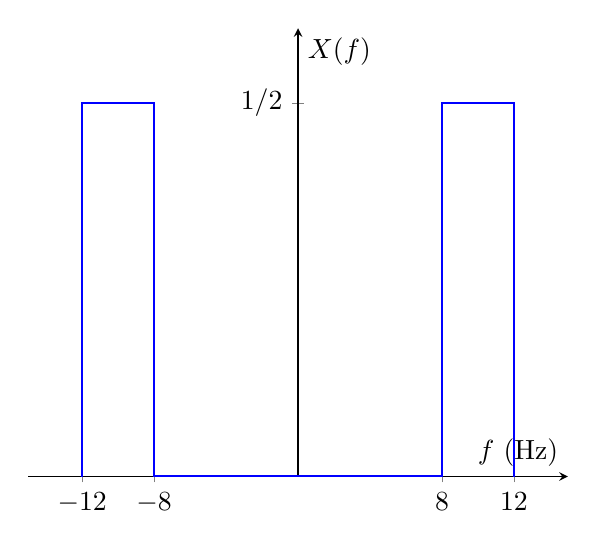
\begin{tikzpicture}
            \begin{axis}[
                axis lines=middle, xlabel=$f$ (Hz), ylabel=$X(f)$,
                xmin=-15, xmax=15, ymin=0, ymax=0.6,
                xtick={-12, -8, 0, 8, 12}, ytick={0.5}, yticklabels={$1/2$}
            ]
            \addplot[blue, thick] coordinates {(-12,0) (-12, 0.5) (-8, 0.5) (-8,0) (8,0) (8, 0.5) (12, 0.5) (12,0)};
            \end{axis}
        \end{tikzpicture}
        \end{center}
        
        \item \textbf{Spettro Campionato e Aliasing}
        
        La condizione di Nyquist ($f_s \ge 2B$) non è soddisfatta, poiché $f_s = 21$ Hz è minore di $2B = 24$ Hz. Ci sarà aliasing. Lo spettro campionato $\tilde{X}(f)$ è una somma di repliche di $X(f)$, scalate per $f_s=21$. L'altezza dei rettangoli replicati sarà $\frac{1}{2} \cdot 21 = 10.5$.
        
        Le repliche che si sovrappongono nella banda base $[-f_s/2, f_s/2] = [-10.5, 10.5]$ Hz provengono da $k=\pm 1$:
        \begin{itemize}
            \item $k=0$ (originale): Rettangoli in $[-12, -8]$ e $[8, 12]$.
            \item $k=1$ (shiftato di +21 Hz): Il rettangolo da $[-12, -8]$ si sposta in $[9, 13]$.
            \item $k=-1$ (shiftato di -21 Hz): Il rettangolo da $[8, 12]$ si sposta in $[-13, -9]$.
        \end{itemize}

        \begin{center}
        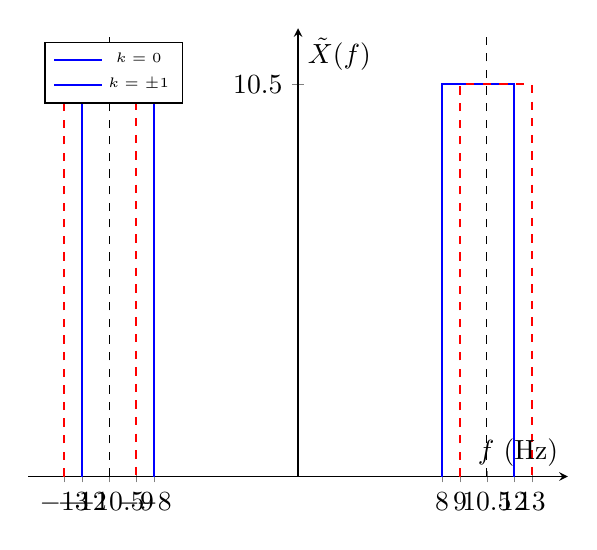
\begin{tikzpicture}
            \begin{axis}[
                axis lines=middle, xlabel=$f$ (Hz), ylabel=$\tilde{X}(f)$,
                xmin=-15, xmax=15, ymin=0, ymax=12,
                xtick={-13,-12, -10.5, -9,-8, 0, 8,9, 10.5, 12,13},
                ytick={10.5}, yticklabels={$10.5$},
                legend pos=north west, legend style={font=\tiny}
            ]
            % Replica k=0
            \addplot[blue, thick] coordinates {(-12,0) (-12, 10.5) (-8, 10.5) (-8,0)};
            \addplot[blue, thick] coordinates {(8,0) (8, 10.5) (12, 10.5) (12,0)};
            \addlegendentry{$k=0$}
            % Replica k=-1
            \addplot[red, thick, dashed] coordinates {(-13,0) (-13, 10.5) (-9, 10.5) (-9,0)};
            \addlegendentry{$k=\pm 1$}
            % Replica k=1
            \addplot[red, thick, dashed] coordinates {(9,0) (9, 10.5) (13, 10.5) (13,0)};
            % Banda di Nyquist
             \draw[dashed, black] (axis cs:-10.5, 0) -- (axis cs:-10.5, 12) node[above, font=\tiny]{$-f_s/2$};
             \draw[dashed, black] (axis cs:10.5, 0) -- (axis cs:10.5, 12) node[above, font=\tiny]{$f_s/2$};
            \end{axis}
        \end{tikzpicture}
        \end{center}
        La sovrapposizione avviene negli intervalli $[-10.5, -9]$ (tra la coda di $k=0$ e $k=-1$) e $[9, 10.5]$ (tra la coda di $k=0$ e $k=1$).

        \item \textbf{Spettro e Segnale Ricostruito}
        
        Il filtro di ricostruzione ideale $H_R(f)$ ha guadagno $T=1/21$ e taglia a $f_c=\pm 10.5$ Hz.
        
        Per calcolare $X_R(f) = \tilde{X}(f) \cdot H_R(f)$, analizziamo il contenuto di $\tilde{X}(f)$ entro la banda $[-10.5, 10.5]$ e lo moltiplichiamo per $1/21$:
        \begin{itemize}
            \item Per $8 \le |f| < 9$: solo la replica $k=0$ contribuisce. Altezza: $10.5 \cdot \frac{1}{21} = 0.5$.
            \item Per $9 \le |f| \le 10.5$: si sommano la replica $k=0$ e quella aliased. Altezza: $(10.5 + 10.5) \cdot \frac{1}{21} = 1$.
        \end{itemize}
        L'espressione analitica di $X_R(f)$ è:
        \[
            \mathbf{X_R(f) = \frac{1}{2}\left[\text{rect}\left(\frac{f}{18}\right) - \text{rect}\left(\frac{f}{16}\right)\right] + 1 \cdot \left[\text{rect}\left(\frac{f}{21}\right) - \text{rect}\left(\frac{f}{18}\right)\right]}
        \]
        (Questa è una forma compatta, ma per l'antitrasformata è meglio vederla come somma di rettangoli centrati).
        $X_R(f)$ è la somma di due coppie di rettangoli:
        \begin{itemize}
            \item $R_1(f)$: due rettangoli di altezza $1/2$ negli intervalli $[-9, -8]$ e $[8, 9]$.
            \item $R_2(f)$: due rettangoli di altezza $1$ negli intervalli $[-10.5, -9]$ e $[9, 10.5]$.
        \end{itemize}
        Antitrasformando, otteniamo una somma di sinc modulati:
        \begin{align*}
            r_1(t) &= \mathcal{F}^{-1}\{R_1(f)\} = \text{sinc}(t) \cdot \cos(2\pi \cdot 8.5t) \\
            r_2(t) &= \mathcal{F}^{-1}\{R_2(f)\} = 1.5 \cdot \text{sinc}(1.5t) \cdot \cos(2\pi \cdot 9.75t)
        \end{align*}
        Il segnale ricostruito finale è la somma dei due:
        \[
            \mathbf{x_R(t) = \text{sinc}(t)\cos(17\pi t) + 1.5\text{sinc}(1.5t)\cos(19.5\pi t)}
        \]
        Il segnale originale è stato quindi irrimediabilmente distorto dall'aliasing.
        
    \end{enumerate}
\end{soluzione}